\section{Proof of the radial law}\label{sec:layer3}
In Section~\ref{sec:unit-circle} we first prove the unit-disk law,
Corollary~\ref{thm:stronglaw}. We then prove
Theorem~\ref{thm:radial-profile} in Section~\ref{sec:moving-radii}, by
the same construction at the moving radii $1+x/n$.

\subsection{The unit circle}\label{sec:unit-circle}
\begin{proof}[Proof of Corollary~\ref{thm:stronglaw}]
The idea is to compare every degree $n$ in a block
$j^8\le n\le(j+1)^8$ with the first degree $N=j^8$ of the block, by root
matching (Theorem~\ref{thm:T4}). A root of $f_N$ is matched unless it
lies outside the annulus $||z|-1|\le K/N$ or has a small derivative
there, and a matched root can cross the unit circle only if its domain
meets that circle.

\emph{Step 1: parameters.}
Fix an integer $K\ge2$. We compare the degrees
$N=j^8\le n\le(j+1)^8=N+m_j$.
In this proof the annulus is $||z|-1|\le K/N$, and, as in
Section~\ref{sec:derivative-detection}, $L=N^{1/64}$.
For the appended tails, let $\rho$ and $a$ be as in
Lemma~\ref{lem:tails}, with $K+2$ in place of $K$ and $m_{\max}=m_j$:
\[
 \rho=1+\frac{K+2}{N},\qquad
 a=15e^{2(K+2)}\sqrt{m_j\log N}.
\]
This lemma bounds every partial tail by $a$ on $|z|\le\rho$.
We write $M_2$ for the bound \eqref{eq:sign-second-derivative} of
Lemma~\ref{lem:second-derivative} on $|f_N''|$ over $|z|\le1+(K+1)/N$, and
$d_0$ for the derivative level of Lemma~\ref{lem:small-derivatives},
below which that lemma counts the annular roots in $B_{K,N}$:
\[
 M_2=100e^{K+4}N^{5/2}\sqrt{\log N},\qquad d_0=N^{3/2}/L.
\]
These parameters must satisfy the conditions of
Table~\ref{tab:unit-conditions}. All of them hold for $N$ beyond a
threshold that depends only on $K$, since the block exponent $8$ makes
$m_j$ of order $N^{7/8}$, and hence $a$ of order $N^{7/16}\sqrt{\log N}$,
while $d_0=N^{3/2-1/64}$.

\begin{table}[ht]
\centering
\small
\begin{tabular}{@{}l>{\raggedright\arraybackslash}p{0.46\textwidth}l@{}}
\toprule
Condition & Needed for & Holds by\\
\midrule
$m_j\le N$ & Lemma~\ref{lem:tails}
 & \eqref{eq:unit-block-length} and $N^{1/8}=j\ge9$\\
$N\ge K+2$ & Lemma~\ref{lem:tails} & large $j$\\
$2a/d_0\le1/N$ & Step~2: the disk of radius $2a/d_0$ about an annular
 root lies in $|z|\le1+(K+1)/N$, where $|f_N''|\le M_2$
 & \eqref{eq:unit-radius-scaled}\\
$4M_2a\le d_0^2$ & Step~2: the hypothesis of
 Lemma~\ref{lem:isolation-interface} & \eqref{eq:unit-parameters}\\
$2a/d_0<N^{-65/64}$ & Step~3: the half-width $N^{-65/64}$ of the thin
 band & \eqref{eq:unit-radius-ratio}\\
\bottomrule
\end{tabular}
\caption{The conditions on the parameters of Step~1 in
Section~\ref{sec:unit-circle}, which hold for all large $j$.}
\label{tab:unit-conditions}
\end{table}

With blocks $j^\beta$ in place of $j^8$, $m_j$ would be of order
$N^{1-1/\beta}$, and $2a/d_0$ and $4M_2a/d_0^2$ of orders
$N^{(1-1/\beta)/2-95/64}$ and $N^{(1-1/\beta)/2-15/32}$, up to
logarithmic factors, so that Steps~2 and~3 would need
$(1-1/\beta)/2<15/32$, that is, $\beta<16$. On the other hand, the bounds
of order $N^{-3/8}$ on the probabilities of the exceptional events in
Step~5 are summable along $N=j^\beta$ only if $3\beta/8>1$, that is,
$\beta>8/3$. The exponent $8$ lies in this range. More precisely, for
$j\ge60$, we have
\begin{align}
 m_j&=(j+1)^8-j^8\le8(j+1)^7=8\Bigl(1+\frac1j\Bigr)^7N^{7/8}\nonumber\\
 &\le8\Bigl(\frac{61}{60}\Bigr)^7N^{7/8}\le9N^{7/8},
 \label{eq:unit-block-length}\\
 a&\le45e^{2(K+2)}N^{7/16}\sqrt{\log N},\label{eq:unit-amplitude}\\
 \frac{2a}{d_0}
 &=\frac{2a}{N^{3/2-1/64}}
 \le90e^{2(K+2)}N^{7/16+1/64-3/2}\sqrt{\log N}\nonumber\\
 &=90e^{2(K+2)}N^{-67/64}\sqrt{\log N},\label{eq:unit-radius}\\
 \frac{2Na}{d_0}&\le90e^{2(K+2)}N^{-3/64}\sqrt{\log N}\longrightarrow0,
 \label{eq:unit-radius-scaled}\\
 \frac{4M_2a}{d_0^2}
 &=\frac{400e^{K+4}N^{5/2}\sqrt{\log N}\,a}{N^{3-1/32}}
 \le180\cdot100e^{K+4}\,e^{2(K+2)}N^{7/16+1/32-1/2}\log N\nonumber\\
 &=180\cdot100e^{K+4}\,e^{2(K+2)}N^{-1/32}\log N\longrightarrow0.
 \label{eq:unit-parameters}
\end{align}
In \eqref{eq:unit-block-length} we use the mean value theorem for the
eighth power on $[j,j+1]$, $j^7=N^{7/8}$, $j\ge60$ and $8(61/60)^7<9$,
and \eqref{eq:unit-amplitude} follows from it. In the last three bounds
we substitute \eqref{eq:unit-amplitude} and $d_0=N^{3/2-1/64}$.

\emph{Step 2: selected domains.}
We call an annular root $\alpha$, that is, a root of $f_N$ with
$||\alpha|-1|\le K/N$, good if $|f_N'(\alpha)|\ge N^{3/2}/L$.
If $|z-\alpha|\le2a/d_0$, then
$|z|\le|\alpha|+2a/d_0\le1+K/N+1/N=1+(K+1)/N<\rho$, since $2a/d_0\le1/N$
by Step~1.
Hence, outside the exceptional event of
Lemma~\ref{lem:second-derivative}, we have $|f_N''|\le M_2$ throughout
this disk, and Lemma~\ref{lem:isolation-interface}, applied with
$P=f_N$, $|f_N'(\alpha)|\ge d_0$ and $4M_2a\le d_0^2$, shows that the
disk contains exactly one zero and that $|f_N|\ge3a/2$ on its boundary.

Let $b\in(a,3a/2)$ be a common regular level.
By Lemma~\ref{lem:isolation-interface}, applied to the family of good
annular roots with the common amplitude $a$,
the selected components of $\{|f_N|<b\}$ are disjoint smooth bounded
domains. Each contains one zero and lies in its localization
disk, since it is connected, contains its root $\alpha$ and does not meet
the circle $|z-\alpha|=2a/d_0$, where $|f_N|\ge3a/2>b$.
The level may depend on $f_N$, but the estimates hold uniformly for every
regular level in this interval.
For a measurable choice, we take the first rational in $(a,3a/2)$,
in a fixed enumeration, outside the finite set of critical-value moduli.

\emph{Step 3: unselected roots and crossings.}
Let $U_N$ denote the number of unselected roots.
Since every good annular root selects a domain that contains no other
root, the unselected roots are the roots with $||\alpha|-1|>K/N$ and the
annular roots that are not good, which $B_{K,N}$ counts. Consequently,
\begin{align}
 U_N
 &\le\#\{\alpha:f_N(\alpha)=0,\ ||\alpha|-1|>K/N\}+B_{K,N},\nonumber\\
 \frac{U_N}{N}
 &\le\frac{2\log2}{K}+C(K)N^{-1/32}(\log N)^7+N^{-1/32}\nonumber\\
 &=\frac{2\log2}{K}+O_K\bigl(N^{-1/32}(\log N)^7\bigr),
 \label{eq:unit-unselected}
\end{align}
where the first count is bounded by \eqref{eq:sign-annular-mass} of
Corollary~\ref{cor:radial-probability}, and $B_{K,N}\le N^{31/32}$ by
Lemma~\ref{lem:small-derivatives}, outside the exceptional events of these
two results.
Let $c_N$ be the number of selected domains whose closures meet the unit
circle. The root of such a domain lies within $2a/d_0$ of the unit
circle, since the closure lies within $2a/d_0$ of the root and
$||\alpha|-1|\le|\alpha-z|$ for a point $z$ of the closure on the unit
circle. We count these roots with the thin-band bound
\eqref{eq:sign-thin-band} of Corollary~\ref{cor:radial-probability},
which controls $\nu_N$ at the radii $1+qN^{-1-\kappa}$ for
$0<\kappa\le1/64$. We take the largest value $\kappa=1/64$, so that the
two error terms $2N^{-\kappa}$ and $C(K)N^{\kappa-1/32}(\log N)^7$ of
\eqref{eq:sign-thin-band} are both $N^{-1/64}$, up to constants and the
factor $(\log N)^7$, and the band half-width $N^{-1-\kappa}=N^{-65/64}$ is
larger than $2a/d_0$ for large $N$, since $65/64<67/64$.
More precisely, by \eqref{eq:unit-radius} we have
\begin{equation}
 \begin{aligned}
 N^{65/64}\,\frac{2a}{d_0}
 &\le90e^{2(K+2)}N^{-67/64+1+1/64}\sqrt{\log N}\\
 &=90e^{2(K+2)}N^{-1/32}\sqrt{\log N}\longrightarrow0,
 \end{aligned}
 \label{eq:unit-radius-ratio}
\end{equation}
and, once $2a/d_0<N^{-65/64}$,
\begin{equation}
 \begin{aligned}
 c_N
 &\le\#\{\alpha:f_N(\alpha)=0,\ 1-N^{-65/64}<|\alpha|<1+N^{-65/64}\}\\
 &=\#\{\alpha:f_N(\alpha)=0,\ |\alpha|<1+N^{-65/64}\}-\nu_N(1-N^{-65/64})\\
 &\le\nu_N(1+N^{-65/64})-\nu_N(1-N^{-65/64}),
 \end{aligned}
 \label{eq:unit-crossings}
\end{equation}
where the first inequality holds since each such root satisfies
$||\alpha|-1|\le2a/d_0<N^{-65/64}$ and distinct domains have distinct
roots, and the equality since the inner inequality is strict.
We apply \eqref{eq:sign-thin-band} with $\kappa=1/64$ and with $2$ in
place of $K$, which suffices since the five radii $1+qN^{-65/64}$,
$q=-2,\dots,2$, lie within $2N^{-65/64}\le2/N$ of the unit circle. For all
sufficiently large $N$, outside five events, one at each of these radii,
we obtain
\begin{equation}
 \left|\frac{\nu_N(1+qN^{-65/64})}N-\frac12\right|
 \le2N^{-1/64}+C(2)N^{-1/64}(\log N)^7,
 \qquad q=-1,0,1.
 \label{eq:unit-thin-band}
\end{equation}
Dividing \eqref{eq:unit-crossings} by $N$ and centering at $\frac12$, we
obtain, whenever $2a/d_0<N^{-65/64}$,
\begin{equation}
 \begin{aligned}
 \frac{c_N}{N}
 &\le\frac{\nu_N(1+N^{-65/64})-\nu_N(1-N^{-65/64})}N\\
 &=\left(\frac{\nu_N(1+N^{-65/64})}N-\frac12\right)
      -\left(\frac{\nu_N(1-N^{-65/64})}N-\frac12\right)\\
 &\le\left|\frac{\nu_N(1+N^{-65/64})}N-\frac12\right|
      +\left|\frac{\nu_N(1-N^{-65/64})}N-\frac12\right|.
 \end{aligned}
 \label{eq:unit-crossings-centered}
\end{equation}
By the cases $q=\pm1$ of \eqref{eq:unit-thin-band}, it follows that
\[
 \frac{c_N}{N}\le4N^{-1/64}+2C(2)N^{-1/64}(\log N)^7
 =O\bigl(N^{-1/64}(\log N)^7\bigr)=o(1).
\]
By Theorem~\ref{thm:sign-logarithms}, each of the five events has
probability at most the right-hand side of
\eqref{eq:sign-log-concentration} at $K=2$, which is summable along
$N=j^8$, as noted after that theorem.
By the Borel--Cantelli lemma, almost surely only finitely many of these
events occur along $N=j^8$, and hence the case $q=0$ of
\eqref{eq:unit-thin-band} holds for all large $j$. Since its right-hand
side tends to zero, $\nu_N(1)/N\to1/2$ almost surely along $N=j^8$.

\emph{Step 4: comparison within a block.}
For $N<n\le N+m_j$, we write $f_n=f_N+g_{n-N}$, where $g_m$ is as in
Lemma~\ref{lem:tails}, with $K+2$ in place of $K$.
Since that lemma bounds all the partial tails at once, outside its tail
event we have $|g_{n-N}|<a$ on $|z|\le\rho$ simultaneously for all these
$n$, and $|z|\le\rho$ contains the closures of the selected domains by
Step~2.
By Lemma~\ref{lem:isolation-interface}, the selected domains then satisfy
the hypotheses of Theorem~\ref{thm:T4} with $P=f_N$, $G=g_{n-N}$ and
$Q=f_n$. Moreover, $\deg f_n=n$ and $\deg f_N=N$, since
$\epsilon_n,\epsilon_N\ne0$. Each of the $s$ selected domains contains
exactly one root of $f_N$, and the other roots of $f_N$ are the unselected
ones, so that $\deg f_N-s=N-s=U_N$.
By Theorem~\ref{thm:T4}, with degrees $N$ and $n$ and with $r=1$, where
$c(1)=c_N$, we have
\begin{align*}
 \max_{N<n\le N+m_j}|\nu_n(1)-\nu_N(1)|
 &\le\max_{N<n\le N+m_j}
      \bigl\{c_N+(\deg f_N-s)\\
 &\qquad+\max(0,\deg f_n-\deg f_N)\bigr\}\\
 &=\max_{N<n\le N+m_j}\bigl\{c_N+U_N+(n-N)\bigr\}=c_N+U_N+m_j.
\end{align*}
Since $m_j/N\to0$, the bound on $c_N/N$ in Step~3,
\eqref{eq:unit-unselected} and \eqref{eq:unit-block-length} give,
outside the exceptional events of Steps~1--4,
\begin{align*}
 \frac1N\max_{N<n\le N+m_j}|\nu_n(1)-\nu_N(1)|
 &\le\frac{c_N}N+\frac{U_N}N+\frac{m_j}N
 \le O\bigl(N^{-1/64}(\log N)^7\bigr)\\
 &\quad+\frac{2\log2}{K}+O_K\bigl(N^{-1/32}(\log N)^7\bigr)+9N^{-1/8}\\
 &=\frac{2\log2}{K}+o_K(1).
\end{align*}
For every degree $n$ in this block, the matching bound above, which holds
trivially for $n=N$, together with $N\le n$ and $n-N\le m_j$, yields
\begin{align}
 \left|\frac{\nu_n(1)}n-\frac12\right|
 &=\left|\frac Nn\left(\frac{\nu_N(1)}N-\frac12\right)
   +\frac{\nu_n(1)-\nu_N(1)}n-\frac{n-N}{2n}\right|\nonumber\\
 &\le \frac Nn\left|\frac{\nu_N(1)}N-\frac12\right|
       +\frac{c_N+U_N+m_j}{n}+\frac{n-N}{2n}\nonumber\\
 &\le \left|\frac{\nu_N(1)}N-\frac12\right|
       +\frac{c_N+U_N}{N}+\frac{3m_j}{2N}.
 \label{eq:unit-block}
\end{align}

\emph{Step 5: exceptional events, and $K\to\infty$.}
Let $E_{K,j}$ denote the common exceptional event in block $j$, the union
of the events of Table~\ref{tab:unit-events}, where $\Pi_K(N)$ is the
right-hand side of \eqref{eq:sign-log-concentration}. For all large $j$,
\begin{equation}
 \Prob(E_{K,j})
 \le4\Pi_K(N)+5\Pi_2(N)+N^{-3}+2N^{-10}+C(K)N^{-3/8}(\log N)^4.
                                                        \label{eq:unit-failure}
\end{equation}
In this bound the shared local-count and derivative events are counted
once each. We count the maximal-tail event once for the whole block,
since outside it the tail bound of Step~4 holds for all the degrees of
the block simultaneously.
With $N=j^8$ we have
$\Pi_K(j^8)=C(K)j^{-3}+j^{-96}+C(K)j^{-7/2}(8\log j)^{-12}$, since
$N^{-3/8}=j^{-3}$, $N^{-12}=j^{-96}$, $N^{-7/16}=j^{-7/2}$ and
$\log N=8\log j$, and \eqref{eq:unit-failure} reads
\[
 \Prob(E_{K,j})
 \le4\Pi_K(j^8)+5\Pi_2(j^8)+j^{-24}+2j^{-80}+C(K)j^{-3}(8\log j)^4.
\]
Hence, for each fixed $K$, every term of \eqref{eq:unit-failure} is
summable over $j$, since the exponents of $j$ are $-3$, $-96$, $-7/2$,
$-24$ and $-80$, and a power of $\log j$ does not affect the convergence.
In finite form, \eqref{eq:unit-failure} is \eqref{eq:block-failure}
with $R=2$, the width of the five thin-band events, and the root-count
bounds of Step~3 are \eqref{eq:block-unselected} and
\eqref{eq:block-center-crossings}.

\begin{table}[ht]
\centering
\small
\setlength{\tabcolsep}{4pt}
\begin{tabular}{@{}llll@{}}
\toprule
Event & Source & Used in & Probability\\
\midrule
Four radial events & \eqref{eq:sign-annular-mass}
 & Step~3, $U_N$ & $\Pi_K(N)$ each\\
Five thin-band events & \eqref{eq:sign-thin-band}, width $2$
 & Step~3, $c_N$, $\nu_N(1)$ & $\Pi_2(N)$ each\\
Local-count event & Lemma~\ref{lem:local-counts}
 & Step~3, $B_{K,N}$ & $N^{-3}$\\
Derivative event & Lemma~\ref{lem:second-derivative}
 & Steps~1--3 & $N^{-10}$\\
Mesh-deviation event & Lemma~\ref{lem:small-derivatives}
 & Step~3, $B_{K,N}$ & $C(K)N^{-3/8}(\log N)^4$\\
Maximal-tail event & Lemma~\ref{lem:tails} & Step~4 & $N^{-10}$\\
\bottomrule
\end{tabular}
\caption{The exceptional events whose union is $E_{K,j}$ in Step~5 of
Section~\ref{sec:unit-circle}. The derivative event is the event that
\eqref{eq:sign-second-derivative} fails, and the local-count, derivative
and mesh-deviation events are those of
Lemma~\ref{lem:small-derivatives}.}
\label{tab:unit-events}
\end{table}

Let $\Omega_K=(\limsup_j E_{K,j})^c$.
Since $\limsup_jE_{K,j}\subset\bigcup_{j\ge J}E_{K,j}$ for every $J$,
the summability above gives
$\Prob(\Omega_K^c)\le\lim_{J\to\infty}\sum_{j\ge J}\Prob(E_{K,j})=0$, and
since there are countably many integers $K\ge2$,
$\Prob(\bigcap_{K=2}^\infty\Omega_K)\ge1-\sum_{K=2}^\infty\Prob(\Omega_K^c)=1$.
On this intersection, for each $K\ge2$, all large $j$ and every $n$ with
$N\le n\le N+m_j$, the bounds \eqref{eq:unit-block}, the case $q=0$ of
\eqref{eq:unit-thin-band}, the bound on $c_N/N$ in Step~3,
\eqref{eq:unit-unselected} and \eqref{eq:unit-block-length} imply that
\begin{align*}
 \left|\frac{\nu_n(1)}n-\frac12\right|
 &\le\left|\frac{\nu_N(1)}N-\frac12\right|
      +\frac{c_N}N+\frac{U_N}N+\frac{3m_j}{2N}\\
 &\le2N^{-1/64}+C(2)N^{-1/64}(\log N)^7
      +4N^{-1/64}+2C(2)N^{-1/64}(\log N)^7\\
 &\quad+\frac{2\log2}{K}+C(K)N^{-1/32}(\log N)^7+N^{-1/32}
      +\frac{27}{2}N^{-1/8}.
\end{align*}
Since every large $n$ lies in such a block, and each term on the right
other than $2\log2/K$ tends to zero as $j\to\infty$, we conclude that
\[
 0\le\limsup_{n\to\infty}\left|\frac{\nu_n(1)}n-\frac12\right|
 \le\inf_{K\ge2}\frac{2\log2}{K}=0.
\]
\end{proof}

\begin{remark}[A deterministic block envelope]\label{rem:block-envelope}
There are deterministic numbers $\varepsilon_j\to0$ and events $E_j$,
defined on the original probability space, such that
$\sum_j\Prob(E_j)<\infty$ and, off $E_j$,
\[
 \max_{j^8\le n<(j+1)^8}\frac{|\nu_n(1)-\nu_{j^8}(1)|}{j^8}\le\varepsilon_j.
\]
\end{remark}

\begin{proof}
We apply Lemma~\ref{lem:deterministic-diagonalization} with the exponent
$8$, $n_j=j^8$ and $X_n=\nu_n(1)$, for which its conclusion is the
assertion of the remark. It requires, for each positive integer $k$,
numbers $a_k$, $b_k(j)$ and $p_k(j)$ such that, for every $j$,
\[
 \Prob\left\{\max_{n_j\le n<n_{j+1}}\frac{|X_n-X_{n_j}|}{n_j}
 >a_k+b_k(j)\right\}\le p_k(j),
\]
where $a_k\to0$ as $k\to\infty$, and where $b_k(j)\to0$ as $j\to\infty$
and $\sum_jp_k(j)<\infty$ for each fixed $k$.

Let $k$ be a positive integer, and put $K=k+1$, so that $K\ge2$, as the
proof of Corollary~\ref{thm:stronglaw} requires. Since every threshold in
that proof depends only on $K$, there is a deterministic $j_0(K)\ge60$
such that for every $j\ge j_0(K)$ the bound \eqref{eq:unit-failure} holds
and, outside the event $E_{K,j}$ of that proof, with $N=j^8$, the
matching bound of Step~4, \eqref{eq:unit-unselected}, the bound on
$c_N/N$ in Step~3 with $C(K)\ge4+2C(2)$, and
\eqref{eq:unit-block-length} give
\begin{align*}
 \max_{N<n\le N+m_j}|\nu_n(1)-\nu_N(1)|&\le c_N+U_N+m_j,\\
 \frac{U_N}N&\le\frac{2\log2}K+C(K)N^{-1/32}(\log N)^7+N^{-1/32},\\
 \frac{c_N}N&\le C(K)N^{-1/64}(\log N)^7,\\
 \frac{m_j}N&\le9N^{-1/8}.
\end{align*}
We set $a_k=2\log2/K$,
\[
 b_k(j)=C(K)N^{-1/32}(\log N)^7+N^{-1/32}
   +C(K)N^{-1/64}(\log N)^7+9N^{-1/8},
\]
and let $p_k(j)$ be the bound \eqref{eq:unit-failure} for
$\Prob(E_{K,j})$ when $j\ge j_0(K)$, and $p_k(j)=1$ when
$j<j_0(K)$.
Since the block $n_j\le n<n_{j+1}$ is contained in $N\le n\le N+m_j$,
and the increment vanishes at $n=N$, the four bounds above give, for
$j\ge j_0(K)$ and outside $E_{K,j}$,
\begin{align*}
 \max_{n_j\le n<n_{j+1}}\frac{|X_n-X_{n_j}|}{n_j}
 &\le\frac1N\max_{N<n\le N+m_j}|\nu_n(1)-\nu_N(1)|\\
 &\le\frac{c_N}N+\frac{U_N}N+\frac{m_j}N
 \le a_k+b_k(j).
\end{align*}
Hence the probability in the above requirement is at most
$\Prob(E_{K,j})\le p_k(j)$ when $j\ge j_0(K)$, and at most $1=p_k(j)$
when $j<j_0(K)$. Moreover, $a_k\to0$ as $k\to\infty$, and, for fixed
$k$, $b_k(j)\to0$ as $j\to\infty$ and $\sum_jp_k(j)<\infty$, since only
finitely many of its terms equal one and the others are summable by
Step~5 of that proof.
By Lemma~\ref{lem:deterministic-diagonalization}, there are therefore
deterministic $\varepsilon_j\to0$ and events $E_j$ with
$\sum_j\Prob(E_j)<\infty$, off which the normalized block increment is at
most $\varepsilon_j$. We may take $E_j$ to be the event on which the
normalized block increment exceeds $\varepsilon_j$, since it is contained
in the event given by the lemma. (In the proof of
Lemma~\ref{lem:deterministic-diagonalization} the given events are this
event for $j\ge J_1$ and $\Omega$ for $j<J_1$, where $J_1$ is the first of
the integers $J_k$ chosen there, and $\sum_{j\ge J_1}\Prob(E_j)\le1$.)
All the events here are defined through the random signs on
the original probability space.
\end{proof}

With $n_j=j^8$ and $X_n=\nu_n(1)$, the numbers $\varepsilon_j$ and the
events $E_j$ of Remark~\ref{rem:block-envelope} are those required by
Theorem~\ref{thm:T5}.

Figure~\ref{fig:root-matching} shows one block, from degree 1000 to
degree 1421, of the sequence with seed 522000.

\begin{figure}[t]
\centering
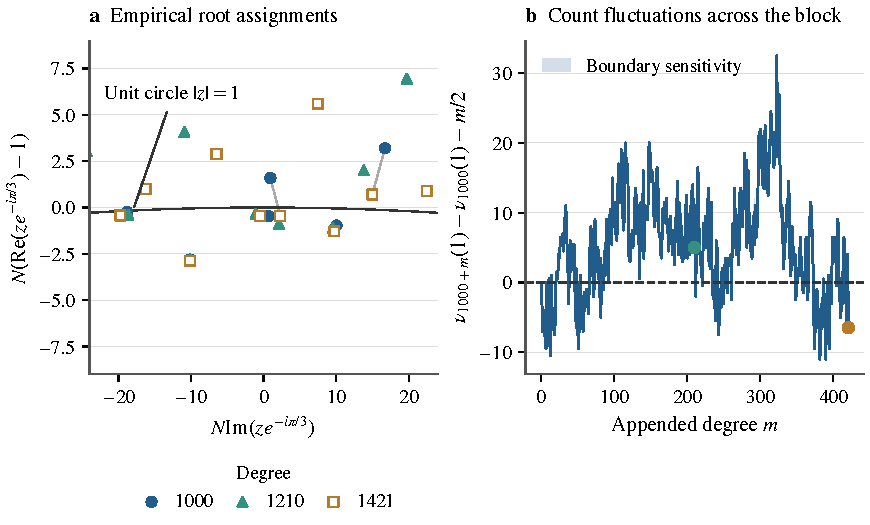
\includegraphics[width=\textwidth]{../numerics/publication/figures/root-matching.pdf}
\caption{Zeros of one sequence at degrees 1000, 1210 and 1421 near
$e^{i\pi/3}$, joined by an uncertified empirical assignment (a), and the
change in the count across the block (b).}
\label{fig:root-matching}
\end{figure}



\subsection{Moving radii}\label{sec:moving-radii}
\begin{proof}[Proof of Theorem~\ref{thm:radial-profile}]
The idea is to repeat the construction of Section~\ref{sec:unit-circle}
with the unit circle replaced by the circle of radius $1+x/N$, for one
$x$ at a time, comparing the degrees in a block by
Corollary~\ref{cor:T4-two-radii}, and then to pass to all $x$ by
monotonicity.

The profile in Proposition~\ref{prop:profiles} satisfies
\[
 F'=\Phi,\qquad 0\le\Phi\le1,\qquad
 0\le\Phi'=2\operatorname{Var}_x(t)\le\frac12.
\]
Here $F'=\Phi$ is part of Proposition~\ref{prop:profiles}, and
$0\le\Phi\le1$ since, by its definition in
Theorem~\ref{thm:radial-profile}, $\Phi(x)$ is the mean of $t$ under the
probability density proportional to $e^{2xt}$ on $[0,1]$. By
\eqref{eq:Phi-variance} in the proof of Lemma~\ref{lem:annular-mass},
$\Phi'(x)=2\operatorname{Var}_x(t)$, where $\operatorname{Var}_x(t)$ is
the variance of $t$ under the same density, and since the variance is at
most the mean square deviation from $\frac12$,
\[
 \operatorname{Var}_x(t)
 \le\frac{\int_0^1(t-\frac12)^2e^{2xt}\dd t}{\int_0^1e^{2xt}\dd t}
 \le\frac14.
\]

Fix $x$ and an integer $R\ge|x|+3$. We use the logarithmic bounds at the
radii $1+(x+qh)/N$, $|q|\le2$, for an offset $h\in(0,1]$ that must meet
the three requirements of Table~\ref{tab:moving-offset}, for the annular
width $K$ fixed below. The value $h=N^{-1/64}$ meets them, since the
quantities in the last column of that table tend to zero. For the first
degree $N=j^8$ of a block, we therefore set
\[
 h=N^{-1/64},\qquad r_N=1+x/N.
\]

\begin{table}[ht]
\centering
\small
\begin{tabular}{@{}>{\raggedright\arraybackslash}p{0.31\textwidth}
>{\raggedright\arraybackslash}p{0.43\textwidth}
>{\raggedright\arraybackslash}p{0.2\textwidth}@{}}
\toprule
Requirement & Reason & At $h=N^{-1/64}$\\
\midrule
$h\to0$ & the secants of $F$ over steps of length $h$ approximate
 $\Phi(x)$ with an error of order $h$ & $N^{-1/64}$\\[2pt]
$N^{-1/32}(\log N)^7/h\to0$ & the secants divide the logarithmic error
 $N^{-1/32}(\log N)^7$ of Theorem~\ref{thm:sign-logarithms} by $h$
 & $N^{-1/64}(\log N)^7$\\[2pt]
$h/N$ exceeds a bound of order $N^{-67/64}\sqrt{\log N}+N^{-9/8}$
 & the band of half-width $h/N$ about $|z|=1+x/N$ contains the root of
 every selected domain that meets the annulus between $|z|=1+x/N$ and
 $|z|=1+x/n$, for every degree $n$ of the block
 & $N^{-1/32}\sqrt{\log N}$ and $N^{-7/64}$\\
\bottomrule
\end{tabular}
\caption{The requirements on the offset $h$ in the proof of
Theorem~\ref{thm:radial-profile}, for fixed $K$ and $x$. The last column
gives $h$, the quotient in the first column, and the two terms of the
bound divided by $h/N$.}
\label{tab:moving-offset}
\end{table}

We apply Theorem~\ref{thm:sign-logarithms}, with $R$ in place of $K$, at
the five radii $r_q=1+y_q/N$, where $y_q=x+qh$ and $q=-2,-1,0,1,2$.
Since $h\le1$, we have $|y_q|\le|x|+2h<R$, so that every $r_q$ lies in
$[1-R/N,1+R/N]$. For all sufficiently large $N$, outside five exceptional
events, one at each radius $r_q$, this theorem gives
$|J_N(r_q)-\log\sigma_N(r_q)+\gamma/2|\le C(R)N^{-1/32}(\log N)^7$, and,
for $N\ge2R$, Lemma~\ref{lem:profile-rate} with $R$ in place of $K$ gives
$|\log\sigma_N(r_q)-\frac12\log N-F(y_q)|\le(R^2+e^{4R}/2)/N$. Adding the
two bounds, and using $1/N\le N^{-1/32}(\log N)^7$ for $N\ge3$, we get,
outside the five exceptional events,
\begin{align}
 \left|J_N(r_q)-\frac12\log N+\frac\gamma2-F(y_q)\right|
 &\le C(R)N^{-1/32}(\log N)^7+\frac{R^2+e^{4R}/2}N\nonumber\\
 &\le\eta_N:=(C(R)+R^2+e^{4R}/2)N^{-1/32}(\log N)^7.
 \label{eq:moving-probes}
\end{align}
For $q=-1,0,1$ we apply Lemma~\ref{lem:local-radial-secant} at $y_q$,
with $R$ in place of $K$, the centering $\frac12\log N$, the profile $F$
of Proposition~\ref{prop:profiles}, $M_F=1/2$ and $B_F=1$, which hold by
the bounds on $\Phi=F'$ above. Its logarithmic error is
$\eta_{\log}=C(R)N^{-1/32}(\log N)^7$, by
Theorem~\ref{thm:sign-logarithms} with $\E\log|G|=-\gamma/2$, and its
profile error is $\varepsilon=(R^2+e^{4R}/2)/N$, by
Lemma~\ref{lem:profile-rate} on $[-R,R]$ for $N\ge2R$, so that
$\eta_{\log}+\varepsilon\le\eta_N$ as in \eqref{eq:moving-probes}. The
lemma applies: outside the five exceptional events $J_N(r_q)$ is finite,
so that $f_N$ is nonzero; $|y_q|+h\le|x|+2h<R<N$, the last since
$N\ge2R$; and its three radii $1+(y_q-h)/N$, $r_q$ and $1+(y_q+h)/N$ are
among the five radii $r_{q'}$. Outside the five exceptional events it
gives
\[
 \left|\frac{\nu_N(r_q)}N-\Phi(y_q)\right|
 \le\frac h4+\frac RN+\frac{2\eta_N(1+R/N)}h.
\]
Since $|\Phi(y_q)-\Phi(x)|\le|q|h/2$ by $0\le\Phi'\le1/2$, since
$|q|h/2+h/4\le2h$ for $|q|\le1$ and $1+R/N\le2$, and since
$r_N+qh/N=r_q$, it follows that, for $q=-1,0,1$,
\begin{align}
 \left|\frac{\nu_N(r_N+qh/N)}N-\Phi(x)\right|
 &\le\frac{|q|h}{2}+\frac h4+\frac RN
       +\frac{2\eta_N(1+R/N)}h\nonumber\\
 &\le\varepsilon_N:=2h+\frac RN+\frac{4\eta_N}h\nonumber\\
 &=2N^{-1/64}+\frac RN+4(C(R)+R^2+e^{4R}/2)N^{-1/64}(\log N)^7\nonumber\\
 &=O_R\bigl(N^{-1/64}(\log N)^7\bigr).
 \label{eq:moving-secant}
\end{align}
Explicit constants for this estimate are given in \eqref{eq:E1-local}.
Moreover, the probabilities of the five logarithmic exceptional events
are summable along $N=j^8$, and $\varepsilon_N\to0$.
Subtracting the two endpoint counts and using \eqref{eq:moving-secant}
with $q=\pm1$, we get
\begin{align}
 &\#\{\alpha:f_N(\alpha)=0,\ ||\alpha|-r_N|<h/N\}\nonumber\\
 &\qquad=\#\{\alpha:f_N(\alpha)=0,\ |\alpha|<r_N+h/N\}-\nu_N(r_N-h/N)\nonumber\\
 &\qquad\le\nu_N(r_N+h/N)-\nu_N(r_N-h/N)\nonumber\\
 &\qquad=N\left(\frac{\nu_N(r_N+h/N)}N-\Phi(x)\right)
   +N\left(\Phi(x)-\frac{\nu_N(r_N-h/N)}N\right)\nonumber\\
 &\qquad\le2\varepsilon_NN,
 \label{eq:moving-band}
\end{align}
where the first equality holds since the inner inequality is strict.

Fix an integer annular width $K\ge R$, and let $a$, $\rho$, $d_0$, the
common regular level $b\in(a,3a/2)$ and the selected domains be those of
Steps~1 and~2 of Section~\ref{sec:unit-circle} at this width.
By Step~2, each selected domain contains exactly one root $\alpha$ of
$f_N$, and its closure lies in the closed disk of radius $2a/d_0$ about
$\alpha$, where $2a/d_0$ is bounded by \eqref{eq:unit-radius}.
For $N\le n\le N+m_j$, with $m_j=(j+1)^8-j^8$ as in Step~1 of
Section~\ref{sec:unit-circle}, the target radius moves by
$|(1+x/n)-(1+x/N)|=|x|(n-N)/(nN)\le|x|m_j/N^2$, and $m_j\le9N^{7/8}$ for
$j\ge60$ by \eqref{eq:unit-block-length}. Since $N/h=N^{65/64}$, these
bounds and \eqref{eq:unit-radius} yield
\begin{align*}
 \frac Nh\left(\frac{2a}{d_0}+\frac{|x|m_j}{N^2}\right)
 &\le90e^{2(K+2)}N^{-67/64+65/64}\sqrt{\log N}+9|x|N^{7/8-2+65/64}\\
 &=90e^{2(K+2)}N^{-1/32}\sqrt{\log N}+9|x|N^{-7/64}
 \longrightarrow0.
\end{align*}
Hence $2a/d_0+|x|m_j/N^2<h/N$ for all $N$ large enough, depending on $K$
and $x$.
Let $D$ be a selected domain whose closure meets the closed annulus
between the circles of radii $r_N$ and $1+x/n$, let $\alpha$ be its root
of $f_N$, and let $z$ be a point of this annulus in the closure of $D$.
Then $|z-\alpha|\le2a/d_0$, and $|z|$ lies between $r_N$ and $1+x/n$, so
that
\begin{align*}
 \bigl||\alpha|-r_N\bigr|
 &\le\bigl||\alpha|-|z|\bigr|+\bigl||z|-r_N\bigr|
 \le|\alpha-z|+\bigl||z|-r_N\bigr|\\
 &\le\frac{2a}{d_0}+\left|\left(1+\frac xn\right)-r_N\right|
 \le\frac{2a}{d_0}+\frac{|x|m_j}{N^2}<\frac hN.
\end{align*}
Hence the root of $f_N$ in such a domain lies in the strict band of
\eqref{eq:moving-band}. This is the case whenever two matched roots lie
on different sides of their respective target circles, since a connected
domain whose closure misses the closed annulus lies inside both circles
or outside both (proof of Corollary~\ref{cor:T4-two-radii}), the
complement of the closed annulus being the union of the disjoint open
sets inside the smaller circle and outside the larger one.
Since distinct domains have distinct roots, by \eqref{eq:moving-band}
the number $c(r_N,1+x/n)$ of these domains is at most $2\varepsilon_NN$.

As in Step~4 of Section~\ref{sec:unit-circle}, outside the tail event of
Lemma~\ref{lem:tails}, with $K+2$ in place of $K$ and $m_{\max}=m_j$, the
appended tail $f_n-f_N$ has modulus less than $a$ on $|z|\le\rho$, which
contains the selected domains, while $|f_N|>a$ on their boundaries. Since
this lemma bounds all the partial tails simultaneously, a single
maximal-tail event controls the entire block and all target radii.
The polynomials $f_N$ and $f_n$ have degrees exactly $N$ and $n$, since
their leading coefficients are $\pm1$, and, with $s$ the number of
selected domains and $U_N$ the number of unselected roots,
$\deg f_N-s=N-s=U_N$, as in Step~4. By
Corollary~\ref{cor:T4-two-radii}, with $P=f_N$, $Q=f_n$, $r=r_N$ and
$r'=1+x/n$, we have
\begin{align*}
 &\max_{N\le n\le N+m_j}|\nu_n(1+x/n)-\nu_N(r_N)|\\
 &\qquad\le\max_{N\le n\le N+m_j}\bigl\{c(r_N,1+x/n)+(\deg f_N-s)
   +\max(0,\deg f_n-\deg f_N)\bigr\}\\
 &\qquad=\max_{N\le n\le N+m_j}\bigl\{c(r_N,1+x/n)+U_N+(n-N)\bigr\}
 \le2\varepsilon_NN+U_N+m_j,
\end{align*}
and $U_N/N$ is bounded by \eqref{eq:unit-unselected} at this width $K$.

Let $E_{K,R,x,j}$ be the union of the events of
Table~\ref{tab:unit-events} at the width $K$, with the five thin-band
events replaced by the five logarithmic events of
Theorem~\ref{thm:sign-logarithms} at the width $R$ and the radii $r_q$.
With $\Pi_K(N)$ as in Step~5 of Section~\ref{sec:unit-circle}, and
$\Pi_R(N)$ the same with $R$ in place of $K$, for all large $j$,
\begin{equation}
 \Prob(E_{K,R,x,j})
 \le4\Pi_K(N)+5\Pi_R(N)+N^{-3}+2N^{-10}+C(K)N^{-3/8}(\log N)^4.
 \label{eq:moving-failure}
\end{equation}
This is \eqref{eq:unit-failure} with $5\Pi_2(N)$ replaced by
$5\Pi_R(N)$, and its finite form is \eqref{eq:block-failure}. At $N=j^8$
its terms are those of Step~5 of Section~\ref{sec:unit-circle} with
$\Pi_R$ in place of $\Pi_2$, so that, for each fixed $K,R,x$, it is
summable over $j$.

For $N\le n\le N+m_j$ we split $\nu_n(1+x/n)/n-\Phi(x)$ into three
terms, and by \eqref{eq:moving-secant} with $q=0$, the matching bound
above, $N\le n\le N+m_j$ and $0\le\Phi\le1$, we have
\begin{align*}
 \left|\frac{\nu_n(1+x/n)}n-\Phi(x)\right|
 &=\biggl|\frac Nn\left(\frac{\nu_N(r_N)}N-\Phi(x)\right)\\
 &\qquad+\frac{\nu_n(1+x/n)-\nu_N(r_N)}n-\frac{n-N}n\Phi(x)\biggr|\\
 &\le \frac Nn\left|\frac{\nu_N(r_N)}N-\Phi(x)\right|
 +\frac{|\nu_n(1+x/n)-\nu_N(r_N)|}{n}\\
 &\quad+\frac{n-N}{n}\Phi(x)
 \le\varepsilon_N+\frac{2\varepsilon_NN+U_N+m_j}N+\frac{m_j}N\\
 &= 3\varepsilon_N+\frac{U_N}N+\frac{2m_j}N.
\end{align*}

Let $\Omega_{K,R,x}=(\limsup_jE_{K,R,x,j})^c$. As in Step~5 of
Section~\ref{sec:unit-circle}, the summability of
\eqref{eq:moving-failure} gives
$\Prob(\Omega_{K,R,x}^c)\le\lim_{J\to\infty}\sum_{j\ge J}\Prob(E_{K,R,x,j})=0$.
On $\Omega_{K,R,x}$ the preceding bounds hold for all large $j$, and
hence, by \eqref{eq:unit-unselected} and $m_j\le9N^{7/8}$, for all large
$j$ and $N\le n\le N+m_j$ we get
\[
 \left|\frac{\nu_n(1+x/n)}n-\Phi(x)\right|
 \le3\varepsilon_N+\frac{2\log2}K+C(K)N^{-1/32}(\log N)^7
 +N^{-1/32}+18N^{-1/8}.
\]
Every large $n$ lies in such a block, and each term on the right other
than $2\log2/K$ tends to zero as $j\to\infty$.
Hence, on the intersection $\Omega_x$ of the events $\Omega_{K,R,x}$ over
integers $K\ge R$, which has probability one as a countable intersection
of events of probability one,
\[
 0\le\limsup_{n\to\infty}
       \left|\frac{\nu_n(1+x/n)}n-\Phi(x)\right|
 \le\frac{2\log2}{K}\longrightarrow0
 \qquad(K\to\infty).
\]
As a countable intersection, the rational event
$\bigcap_{x\in\mathbb Q}\Omega_x$ also has probability one.

For any real $x$, choose rationals $x_-<x<x_+$. By monotonicity we have
$\nu_n(1+x_-/n)/n\le\nu_n(1+x/n)/n\le\nu_n(1+x_+/n)/n$, and taking
limits on the rational event we get
\[
 \Phi(x_-)\le\liminf_{n\to\infty}\frac{\nu_n(1+x/n)}n
 \le\limsup_{n\to\infty}\frac{\nu_n(1+x/n)}n
 \le\Phi(x_+).
\]
Letting $x_-$ increase to $x$ and $x_+$ decrease to $x$ through
rationals, the continuity of $\Phi$ shows that the limit inferior and the
limit superior are both $\Phi(x)$.
To prove the uniform convergence, fix a compact interval $I$ and
$\delta>0$, write $\widehat\Phi_n(x)=\nu_n(1+x/n)/n$, and choose rational
numbers $x_0<x_1<\cdots<x_M$ with $I\subset(x_0,x_M)$ and
$x_{i+1}-x_i<\delta$. For $x\in[x_i,x_{i+1}]\cap I$ we have
\[
 \widehat\Phi_n(x_i)-\Phi(x_{i+1})
 \le\widehat\Phi_n(x)-\Phi(x)
 \le\widehat\Phi_n(x_{i+1})-\Phi(x_i),
\]
since $\widehat\Phi_n$ is nondecreasing, as $\nu_n$ is, and $\Phi$ is
nondecreasing, as $\Phi'\ge0$.
Taking the supremum over $x\in I$, we get
\begin{align*}
 \sup_{x\in I}|\widehat\Phi_n(x)-\Phi(x)|
 &\le \max_{0\le i\le M}|\widehat\Phi_n(x_i)-\Phi(x_i)|
       +\max_{0\le i<M}\{\Phi(x_{i+1})-\Phi(x_i)\}\\
 &\le \max_{0\le i\le M}|\widehat\Phi_n(x_i)-\Phi(x_i)|
       +\frac{\delta}{2},
\end{align*}
where the second inequality follows from $|\Phi'|\le1/2$ and
$x_{i+1}-x_i<\delta$ by the mean value theorem.
On the rational event the maximum tends to zero, and we then let
$\delta$ tend to zero.
Finally, we intersect over intervals with integer endpoints.
All these intersections take place on the given probability space.
Since the rational event does not depend on $I$, the uniform convergence
holds on it for every compact interval $I$ at once, and in particular for
$I=[-A,A]$ for every $A>0$, which is the assertion of
Theorem~\ref{thm:radial-profile}.
\end{proof}
